\def\CTeXPreproc{Created by ctex v0.2.9, don't edit!}
%\documentclass{beamer}
\documentclass[%handout,
xcolor=pdftex]{beamer}
\mode<presentation> {
  \usetheme{Warsaw}
  \setbeamercovered{transparent}
}
\let\Tiny=\tiny
\usetheme{Singapore}
\usecolortheme{dolphin}
\usepackage{amsmath}
\usepackage{textcomp}
\usepackage{amssymb}
\usepackage{amsthm}
\usepackage{graphicx}
\usepackage{color}
\usepackage{lipsum}
\usepackage{hyperref}
\usepackage{multirow}
\usepackage{bm}
\DeclareMathSymbol{\Phi}{\mathalpha}{operators}{8}
%\setbeamertemplate{headline}{}
\setbeamertemplate{footline}[page number]
\newcommand\Fontvi{\fontsize{9pt}{8}\selectfont}
\newcommand\Fontvii{\fontsize{7pt}{8}\selectfont}
\newcommand{\backupbegin}{
   \newcounter{finalframe}
   \setcounter{finalframe}{\value{framenumber}}
}
\newcommand{\backupend}{
   \setcounter{framenumber}{\value{finalframe}}
}\newtheorem{proposition}{Proposition}
\title{Unit 24: Lagged Regression}
\author[STAT 5170: Applied Time Series, Unit 26]{Jeffrey Woo}
\institute{Department of Statistics, University of Virginia}
\date{Spring 2020}

\AtBeginSubsection[] {
  \begin{frame}<beamer>{Outline}
    \tableofcontents[currentsection,currentsubsection]
  \end{frame}
}



\begin{document}


\frame{\titlepage}


\begin{frame}
\frametitle{Readings for Unit 24}

Textbook chapter 1.4 (page 23 to 25), 5.5.

\end{frame}


\begin{frame}
\frametitle{Last Unit}
\begin{enumerate}
\item Linear Regression with AR errors.
\end{enumerate}
\end{frame}

\begin{frame}
\frametitle{Motivation}

We'll explore the lagged regression model: used to identify a relationship between two time series with a lagged effect.


\end{frame}

\section{Bivariate Processes}
\frame{\tableofcontents[currentsection]}

%\begin{frame}
%\frametitle{Lagged Regression Model}

%Lagged regression models take the form

%\begin{equation*}
%y_t = \sum_{h=-\infty}^{\infty} \beta_h x_{t-h} + v_t,
%\end{equation*}

%where $x_t$ is the input time series, $y_t$ is the output time series, and $v_t$ is a stationary noise process. Such models can be used to identify a relationship between two time series and forecast one time series from the other. Lagged versions of the output series are sometimes also considered as inputs.


%\end{frame}

%\begin{frame}
%\frametitle{Lagged Regression Model}

%If we think about the SOI and recruitment datasets that we've looked at, we may want to see how the number of new fish is related to the Southern Oscillation Index (change in air pressure) in the Central Pacific Ocean, or predict future values of the number of new fish from the SOI.

%\end{frame}

%\begin{frame}
%\frametitle{Lagged Regression Model}

%We'll explore both the time domain and frequency domain approaches.

%\end{frame}



\begin{frame}
\frametitle{Bivariate Processes}

Consider the bivariate time series $(x_1,y_1), (x_2, y_2), \cdots (x_n, y_n)$. Define the following:

\begin{itemize}
\item $\mbox{E}(x_t) = \mu_x, \mbox{E}(y_t) = \mu_y$.
\item $\gamma_x (h) = \mbox{Cov}(x_t, x_{t+h}), \gamma_y (h) = \mbox{Cov}(y_t, y_{t+h})$.
\end{itemize}

\end{frame}

\begin{frame}
\frametitle{Cross-Covariance}

The cross-covariance function, $\gamma_{xy}(h)$, measures the strength of the linear relationship between two variables at a certain lag. If $\{x_t\}$ and $\{y_t\}$ are jointly stationary processes, then

\begin{equation} \label{eq:cov}
\gamma_{xy}(h) = \mbox{E}\left[ (x_{t+h} - \mu_x) (y_{t} - \mu_y) \right].
\end{equation}



\end{frame}



%\begin{frame}
%\frametitle{Cross-Covariance}

%However, $\gamma_{xy}(h) = \gamma_{yx}(-h)$.\\
%\vspace{60mm}

%\end{frame}

\begin{frame}
\frametitle{Cross-Covariance}

\begin{itemize}
\item $\gamma_{xy}(h)$: $y_t$ is leading $x_t$.
\item $\gamma_{xy}(-h)$: $x_t$ is leading $y_t$.
\end{itemize}

\vspace{5mm}

\textbf{Toy example:} Consider $x_t$ being the gas input and $y_t$ the CO2 output of a furnace. The fluctuations of $y_t$ is delayed with respect to the fluctuations of $x_t$ due to chemical reaction time for gas to produce CO2.

\end{frame}



\begin{frame}
\frametitle{Cross-Correlation}

The cross-correlation function of jointly stationary $\{x_t\}$ and $\{y_t\}$ is

\begin{equation} \label{eq:cor}
\rho_{xy}(h) = \frac{\gamma_{xy}(h)}{\sqrt{\gamma_x(0) \gamma_y(0)}}.
\end{equation}

Properties:
\begin{itemize}
\item $\rho_{xy}(h) = \rho_{xy}(-h)$.
\item $|\rho_{xy}(h)| \leq 1$.
\end{itemize}

\end{frame}

\begin{frame}
\frametitle{Joint Stationarity}

\textbf{Jointly stationary}: constant means, autocovariances depending only on lag $h$, cross-covariance depends only on lag $h$.\\

\vspace{5mm}

Recall that the autocovariance function is symmetric. The cross-covariance function, $\gamma_{xy}(h)$, is not symmetric, i.e. $\gamma_{xy}(h) \neq \gamma_{xy}(-h)$. However, $\gamma_{xy}(h) = \gamma_{yx}(-h)$.

\end{frame}

\begin{frame}
\frametitle{Worked Example}

Consider the following processes: $x_t = w_t + w_{t-1}$, $y_t = x_t - x_{t-1}$. Derive the cross-covariance function, cross-correlation function, and show that $\{x_t\}$ and $\{y_t\}$ are jointly stationary.\\

\vspace{50mm}

\end{frame}

\begin{frame}
\frametitle{Sample Cross-Covariance and Sample CCF}

Sample cross-covariance

\begin{equation*}
\hat{\gamma}_{xy}(h) = \frac{1}{n} \sum_{i=1}^{n-h} (x_{t+h} - \bar{x}) (y_{t} - \bar{y})
\end{equation*}

for $h \geq 0$. The sample CCF is

\begin{equation*}
\hat{\rho}_{xy}(h) = \frac{\hat{\gamma}_{xy}(h)}{\sqrt{\hat{\gamma}_{x}(0) \hat{\gamma}_{y}(0) }}
\end{equation*}

If $\{x_t\}$ or $\{y_t\}$ is \textbf{white noise}, then $\hat{\rho}_{xy}(h) \sim N(0, 1/n)$.

\end{frame}

\begin{frame}
\frametitle{Prewhitening}

If neither $\{x_t\}$ nor $\{y_t\}$ is white noise, then hypothesis tests to detect significant CCFs are unreliable. Thus, we typically \textbf{prewhiten} the data, then produce the CCF plot of the data. 

\begin{itemize}

\item Prewhitening transforms both variables in a way that the one of the variables becomes white noise after transformation. 

\item We then produce a CCF plot of the data, and can reliably interpret the plot. 

\end{itemize}

\end{frame}

\begin{frame}
\frametitle{Sample Cross-Covariance and Sample CCF}

\textbf{Example}: CCF of SOI and recruit data with prewhitening.

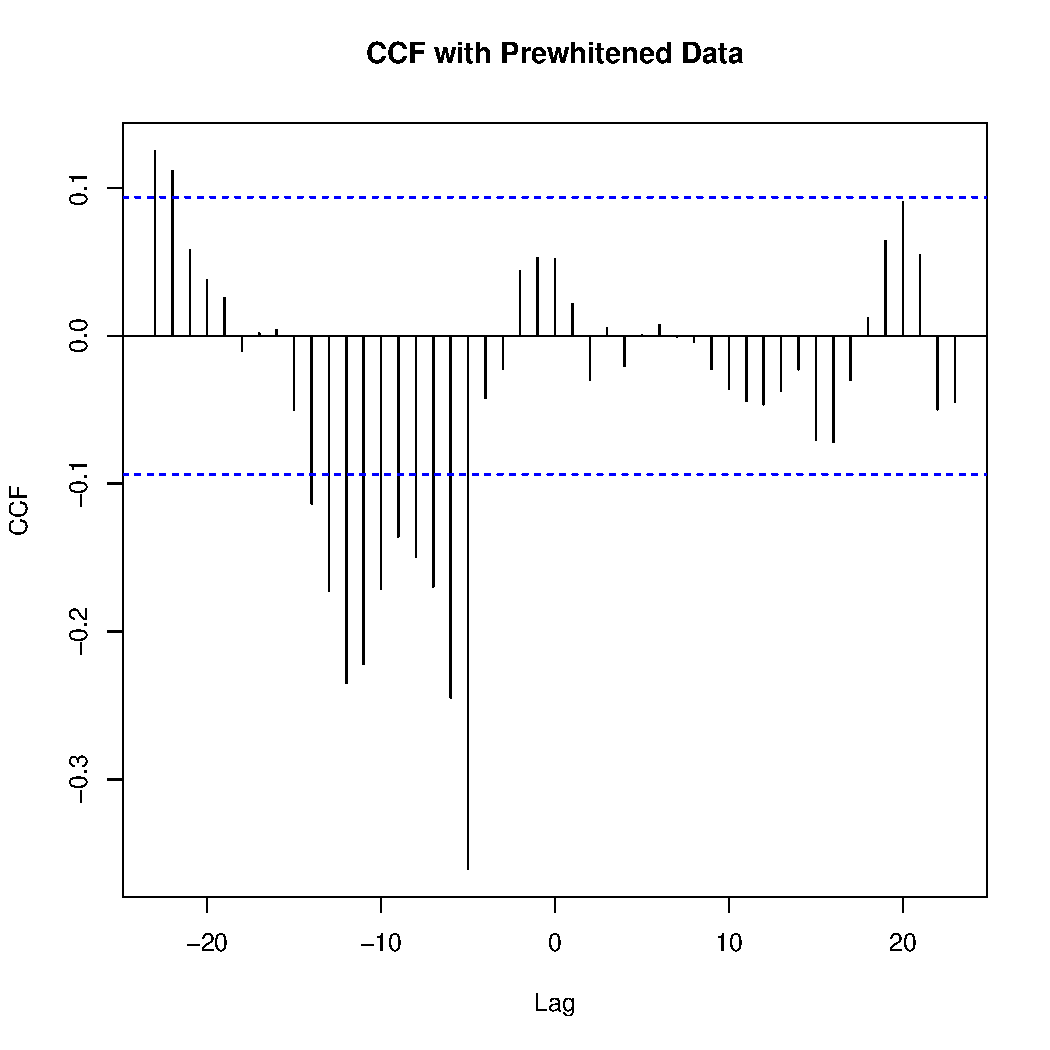
\includegraphics[width=110mm, height=75mm]{ccf_soi.pdf}

\end{frame}

\begin{frame}
\frametitle{Sample Cross-Covariance and Sample CCF}

Peak appears at $h=-5$, this indicates that SOI at time $t-5$ has \textbf{strongest correlation} with recruitment at time $t$. SOI \textbf{leads} recruitment by 5 months. The CCF is negative, which tells us that the two time series move in opposite directions: increase in SOI is associated with a decrease in recruitment.

\end{frame}

\section{Lagged Regression Model}
\frame{\tableofcontents[currentsection]}

\begin{frame}
\frametitle{Lagged Regression Model in Time Domain}

We typically consider lagged regression models of the form

\begin{equation} \label{eq:lag1}
y_t = \sum_{j=0}^\infty \alpha_j x_{t-j} + \eta_t = \alpha(B) x_t + \eta_t
\end{equation}

where $\alpha(B) = \sum_{j=0}^\infty \alpha_j$ and $\eta_t$ is a stationary ARMA noise process. 



\end{frame}





\begin{frame}
\frametitle{Box-Jenkins Approach}

Box \& Jenkins have proposed that $\alpha(B)$ in (\ref{eq:lag1}) can often be expressed as a ratio of polynomials involving a smaller number of coefficients, along with a specific delay, $d$, i.e.

\begin{equation} \label{eq:alpha}
\alpha(B) = \frac{\delta(B) B^d}{\omega(B)},
\end{equation}

where 

\begin{itemize}

\item $\delta(B) = \delta_0 + \delta_1 B + \cdots + \delta_s B^s$ and
\item $\omega(B) = 1 - \omega_1 B - \cdots - \omega_r B^r$.

\end{itemize}

\end{frame}

\begin{frame}
\frametitle{Box-Jenkins Approach}

Subbing (\ref{eq:alpha}) into (\ref{eq:lag1}), we obtain

\begin{equation} \label{eq:lag2}
y_t = \frac{\delta(B) B^d}{\omega(B)} x_t + \eta_t
\end{equation}


\end{frame}

\begin{frame}
\frametitle{Box-Jenkins Approach}

Expanding the backshifts in $\delta(B)$ and $\omega(B)$ in (\ref{eq:lag2}), we obtain

\begin{equation} \label{eq:reg}
y_t = \sum_{k=1}^r \omega_k y_{t-k} + \sum_{k=0}^s \delta_k x_{t-d-k} + u_t.
\end{equation}

where $u_t = \omega(B)\eta_t$.\\

\end{frame}

\begin{frame}
\frametitle{Box-Jenkins Approach}

\begin{itemize}
\item So we perform a regression of $y_t$ on the lagged versions of both $y_t$ and $x_t$ series to obtain the estimates of $\boldsymbol{\beta} = (\omega_1, \cdots, \omega_r, \delta_0, \delta_1, \cdots, \delta_s)$.
\item We normally just consider $u_t$ to be an ARMA process, and use the methods discussed in Unit 23 to estimate $u_t$.
\end{itemize}

\end{frame}


\begin{frame}
\frametitle{Box-Jenkins Methodology for Lagged Regression}

\begin{enumerate}

\item Fit an ARMA model for $x_t$, so we have estimates of $\theta_x(B)$ and $\phi_x(B)$.
\item Prewhiten the variables by applying the operator $\frac{\phi_x(B)}{\theta_x(B)}$ to both variables.
\item Compute the cross-correlation of the variables (after prewhitening) to estimate the time delay $d$ and suggest a form for (\ref{eq:reg}).
\item Obtain $\boldsymbol{\hat{\beta}} = (\hat{\omega}_1, \cdots, \hat{\omega}_r, \hat{\delta}_0, \hat{\delta}_1, \cdots, \hat{\delta}_s)$ using a regression of the form in (\ref{eq:reg}). Store the residuals from this regression.
\item Fit an ARMA model for the noise $u_t$ using the residuals from the previous step and using the techniques mentioned in Unit 23. 

\end{enumerate}

\end{frame}

\begin{frame}
\frametitle{Common Patterns in CCF Plot}

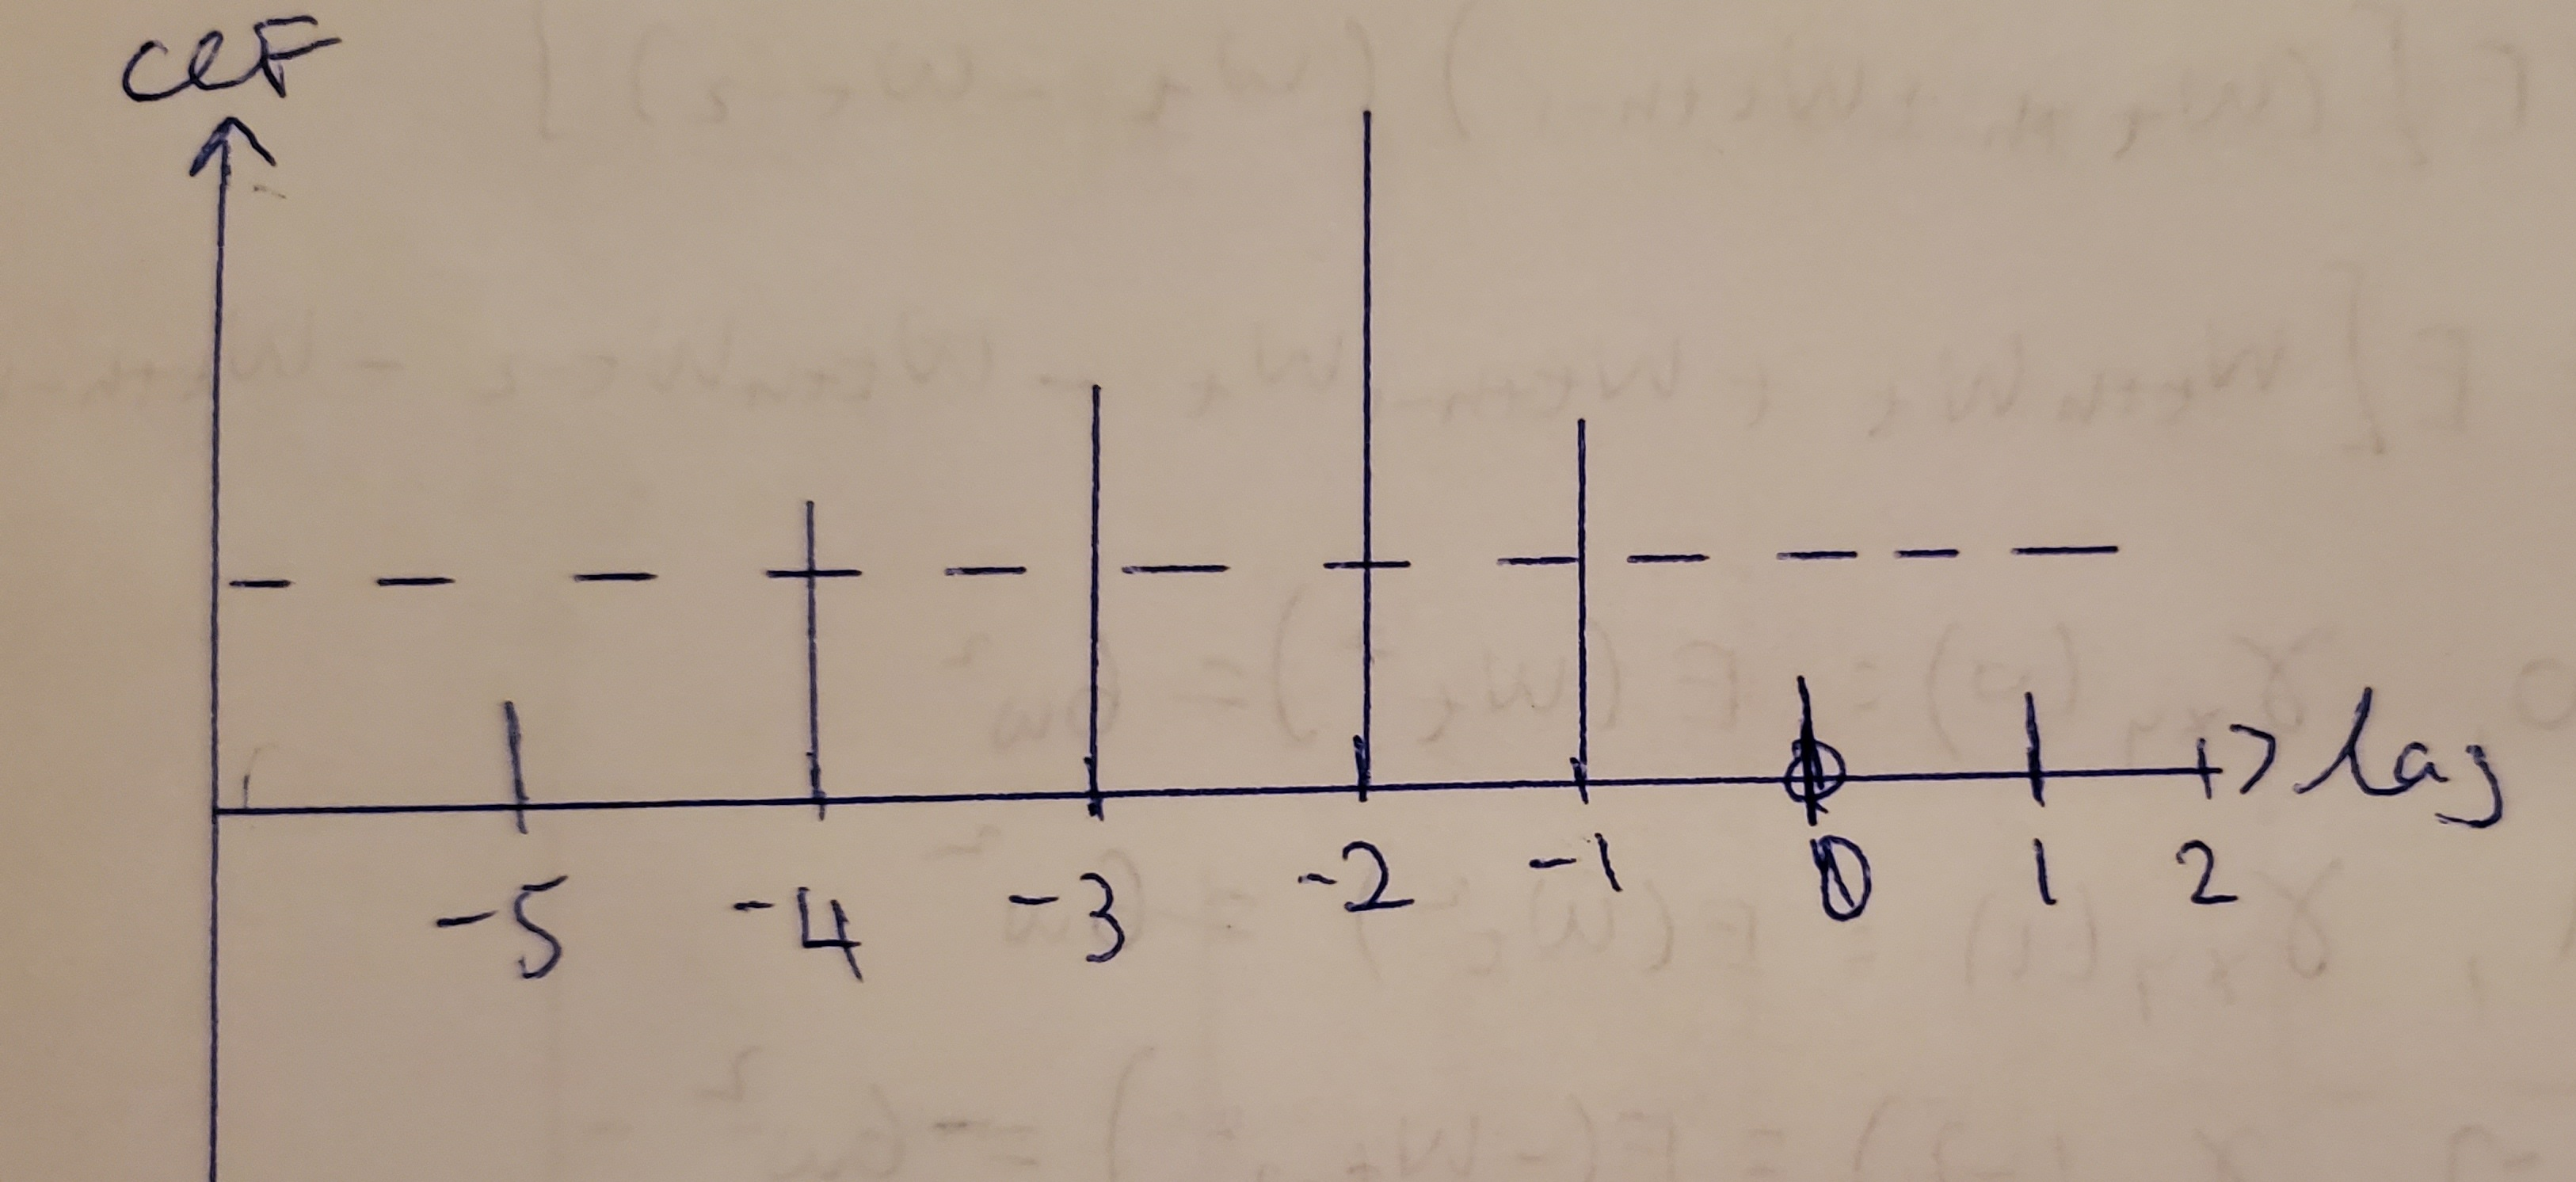
\includegraphics[width=110mm, height=60mm]{slide23.jpg}

\end{frame}

\begin{frame}
\frametitle{Common Patterns in CCF Plot}

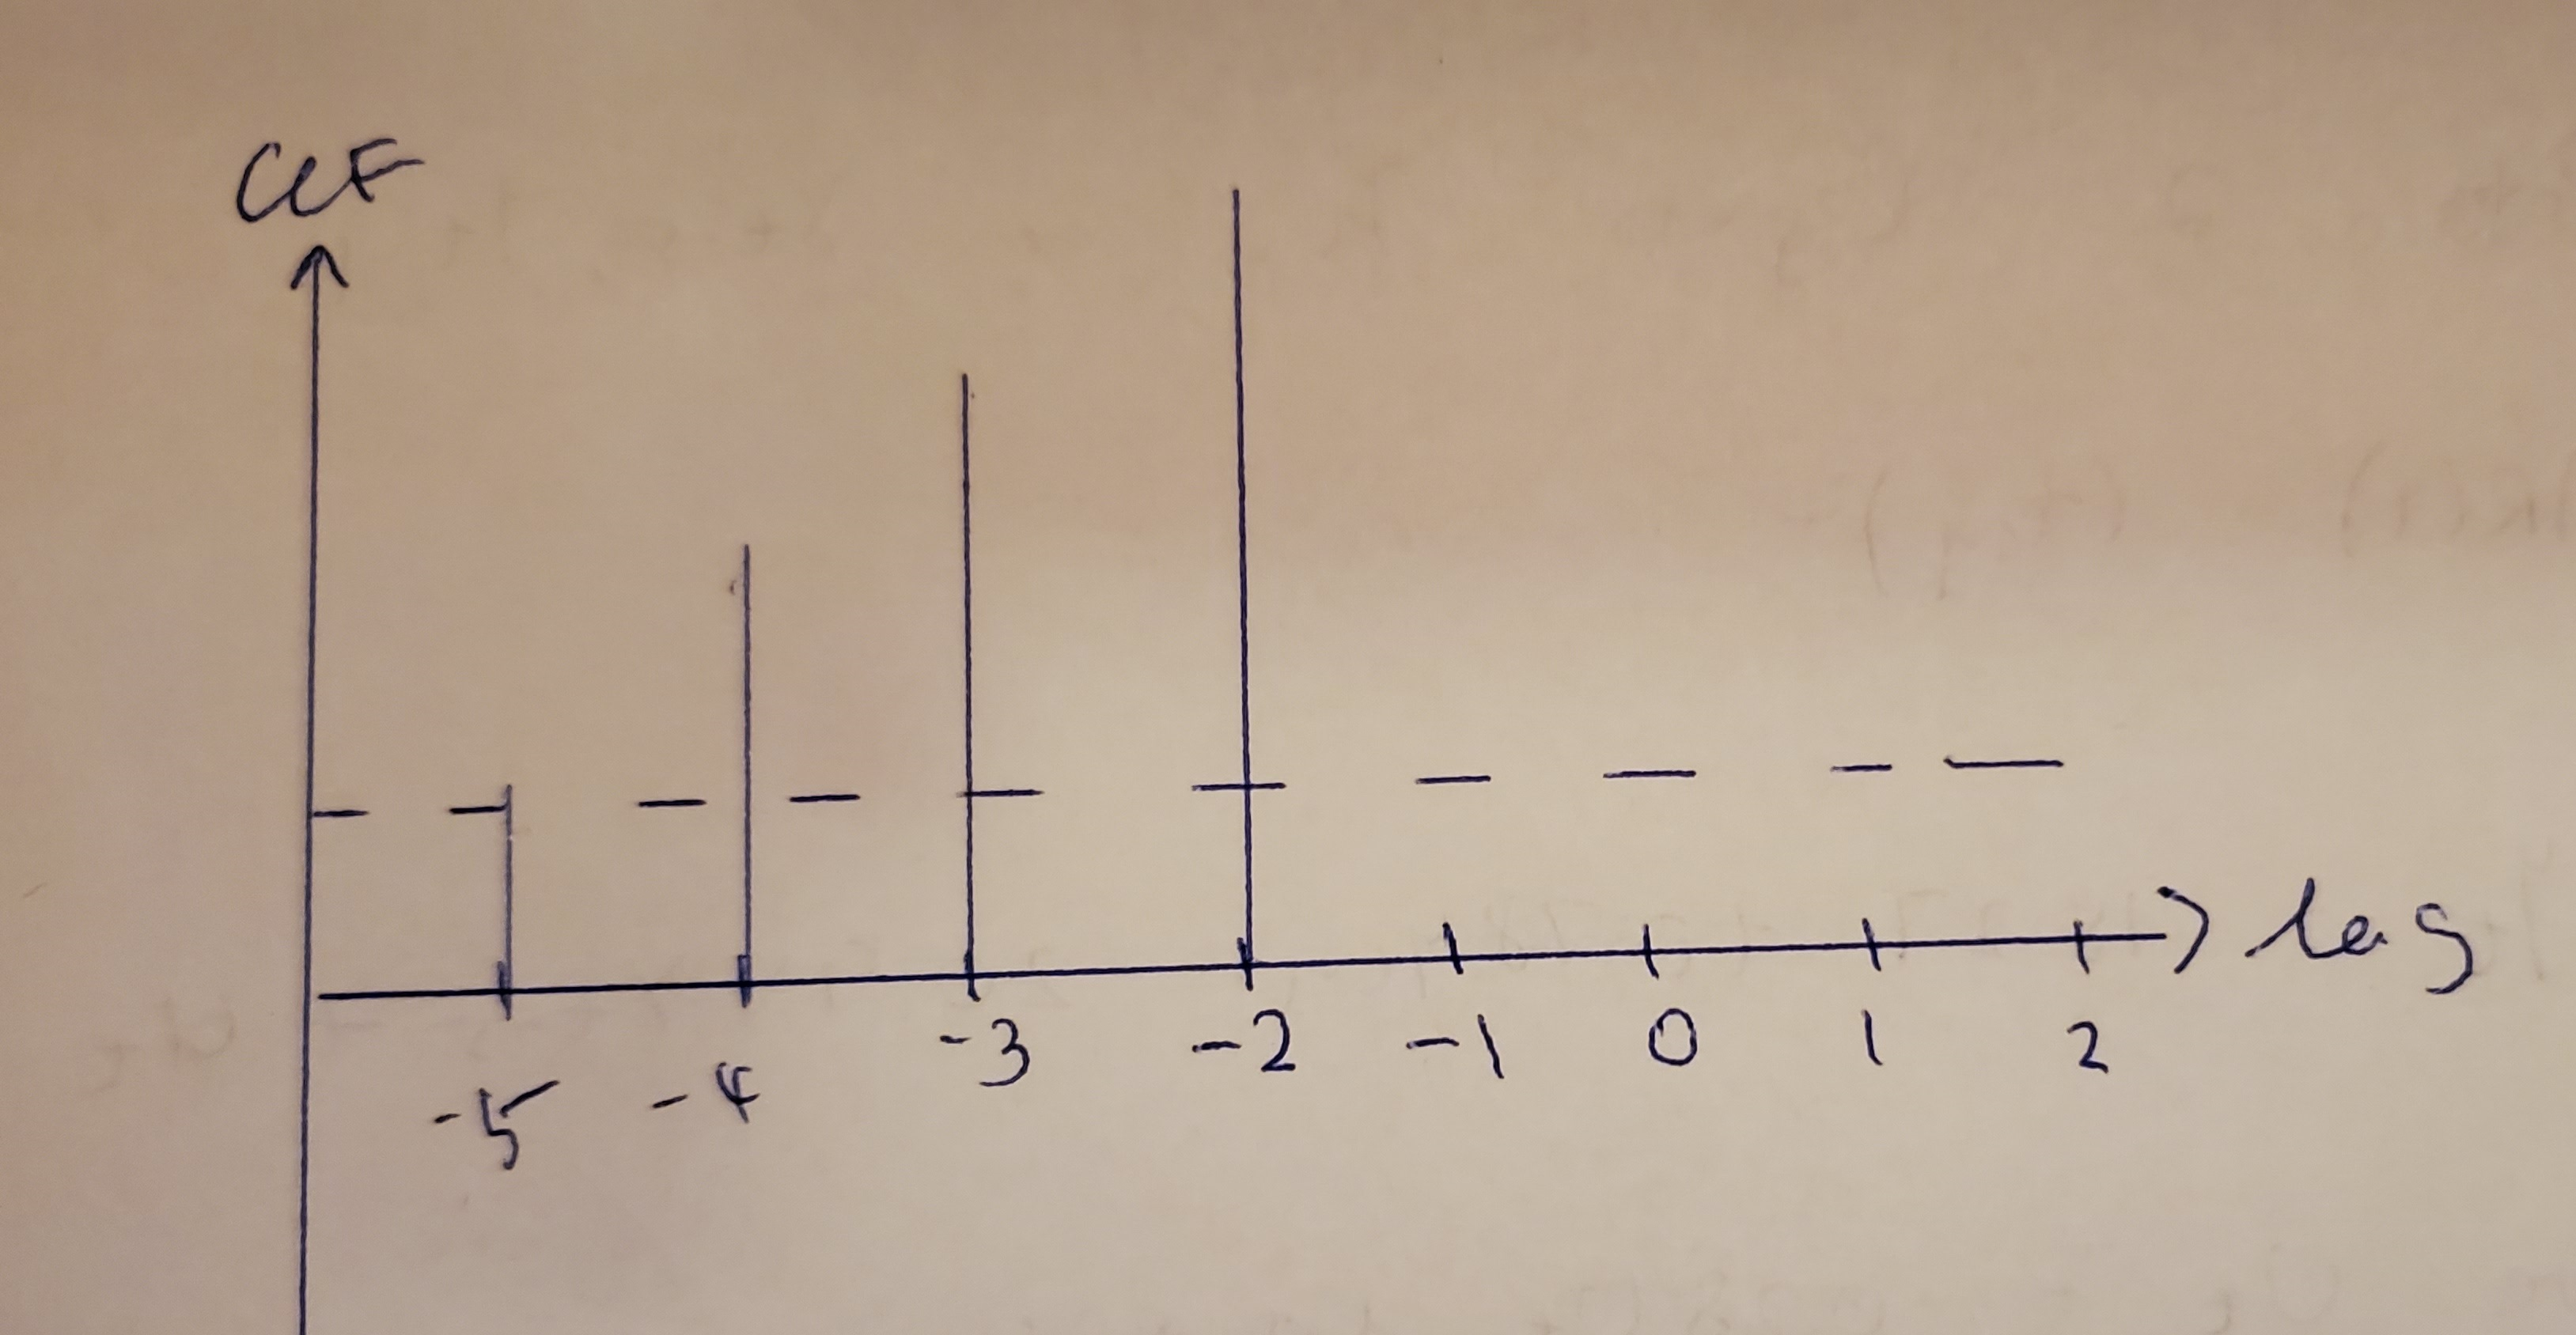
\includegraphics[width=110mm, height=60mm]{slide24.jpg}

\end{frame}

\begin{frame}
\frametitle{Common Patterns in CCF Plot}

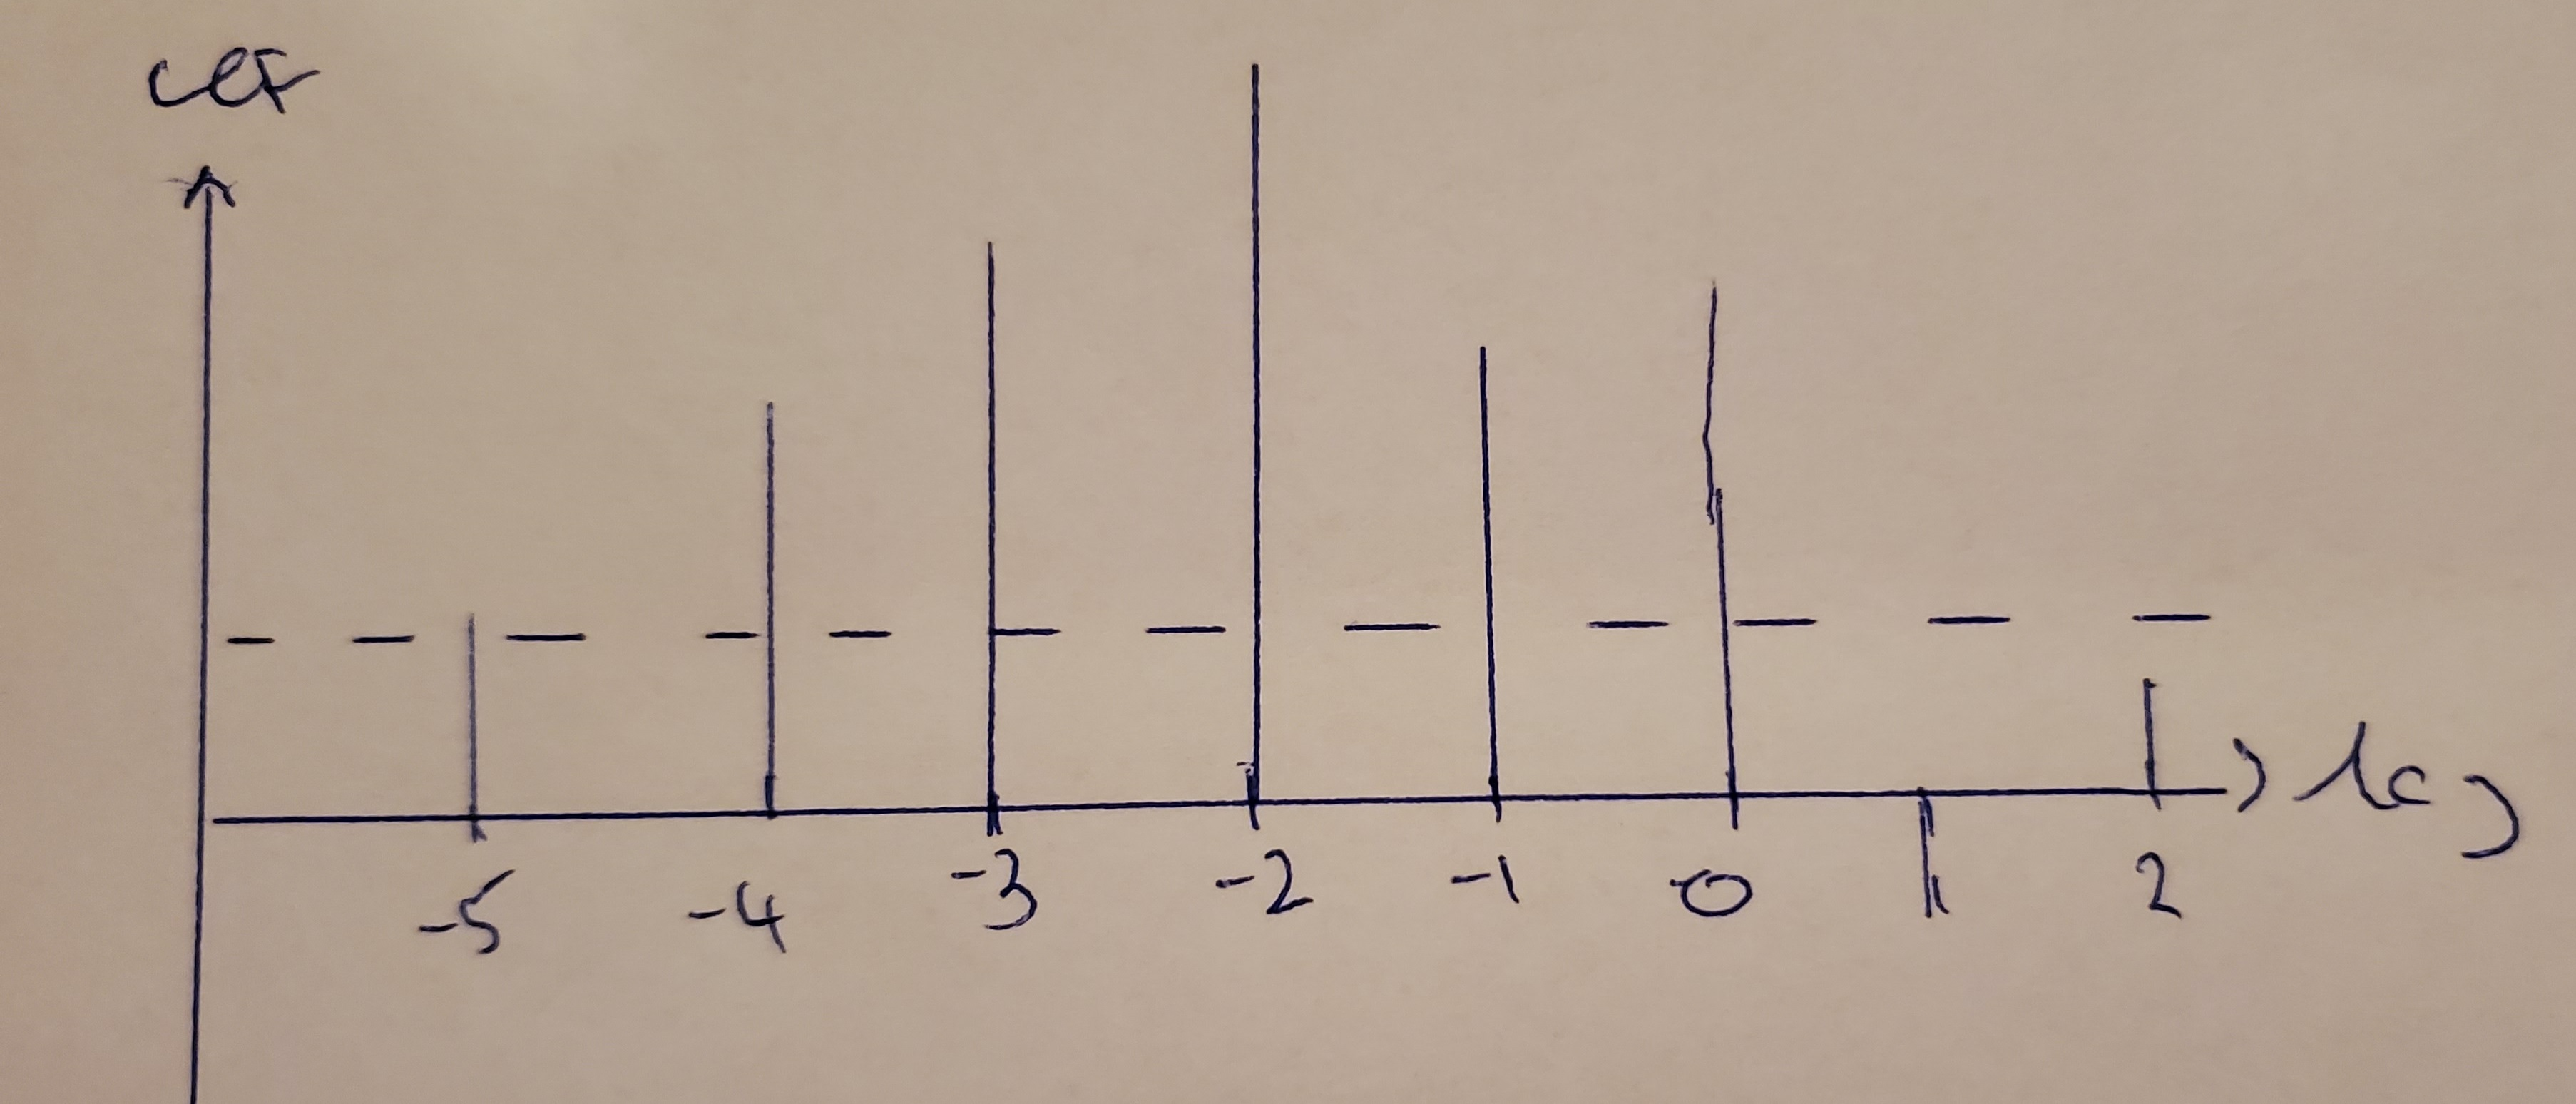
\includegraphics[width=110mm, height=60mm]{slide25.jpg}

\end{frame}



%\begin{frame}
%\frametitle{Lagged Regression Model in Time Domain}

%The prewhitening step inverts the linear filter $x_t = \frac{\theta_x(B)}{\phi_x(B)} w_t$. Then the lagged regression is between the transformed $y_t$ and a white noise series $w_t$. This enables us to determine a suitable lag.

%\end{frame}

\section{Worked Example}
\frame{\tableofcontents[currentsection]}

\begin{frame}
\frametitle{Worked Example}

Some of these steps are worked out in some functions in R. What we still need to do is to examine the prewhitened CCF to determine the kind of lagged regression model we should fit (step 3), and examine residuals to determine their ARMA structure (step 5).


\end{frame}

\begin{frame}
\frametitle{Worked Example}

We will use the Southern Oscillation Index and recruitment datasets, which contain monthly data on the changes in air pressure and estimated number of new fish in the central Pacific Ocean from 1950 to 1987. We wish to fit a lagged regression model (\ref{eq:reg}) for the number of new fish against lagged versions of number of new fish and the change in air pressure in the Central Pacific Ocean. 

\end{frame}

\begin{frame}
\frametitle{Worked Example}

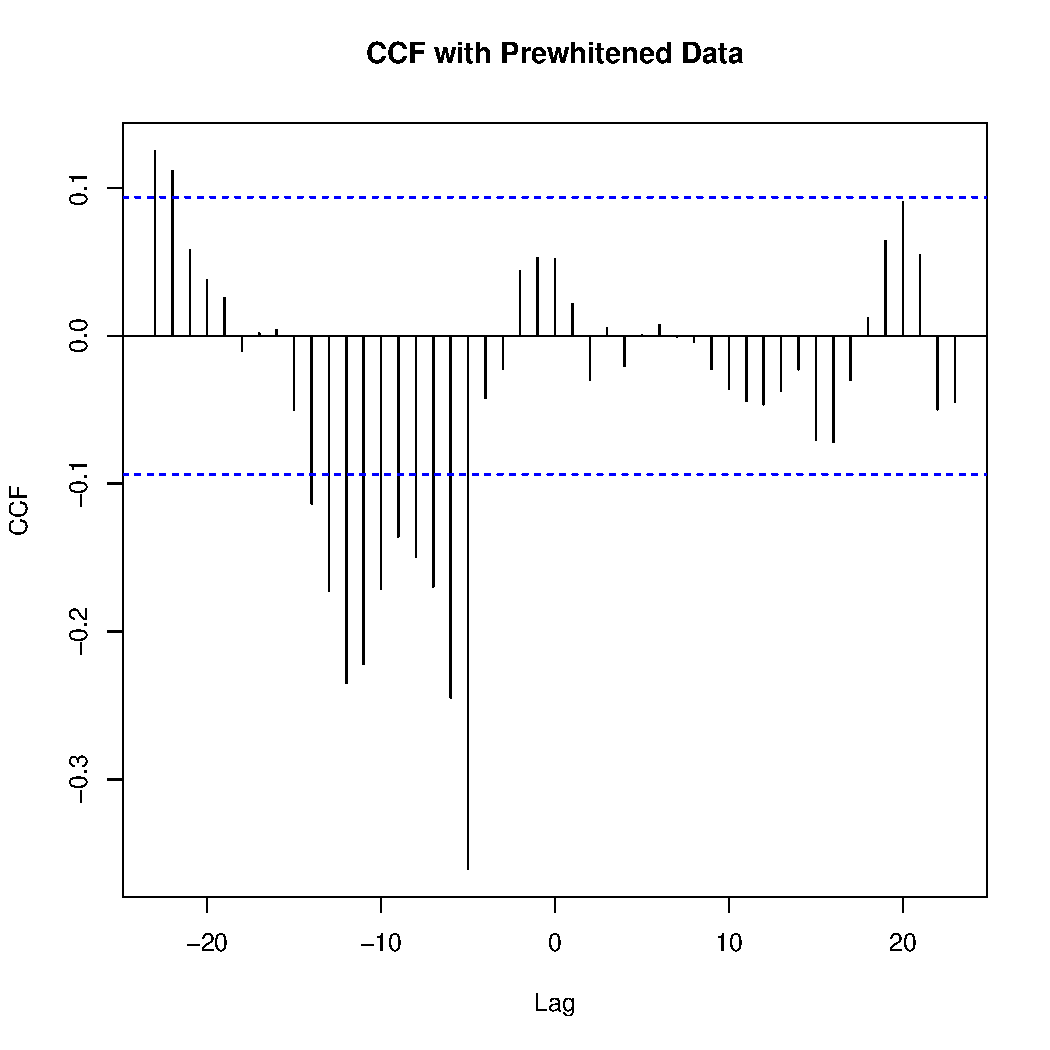
\includegraphics[width=110mm, height=60mm]{ccf_soi.pdf}

What form should (\ref{eq:reg}) take?

\end{frame}

\begin{frame}
\frametitle{Worked Example}

After deciding the appropriate (lagged) regression, fit the model, and examine the ACF and PACF of the residuals to decide their ARMA structure.

\end{frame}

\begin{frame}
\frametitle{Worked Example}

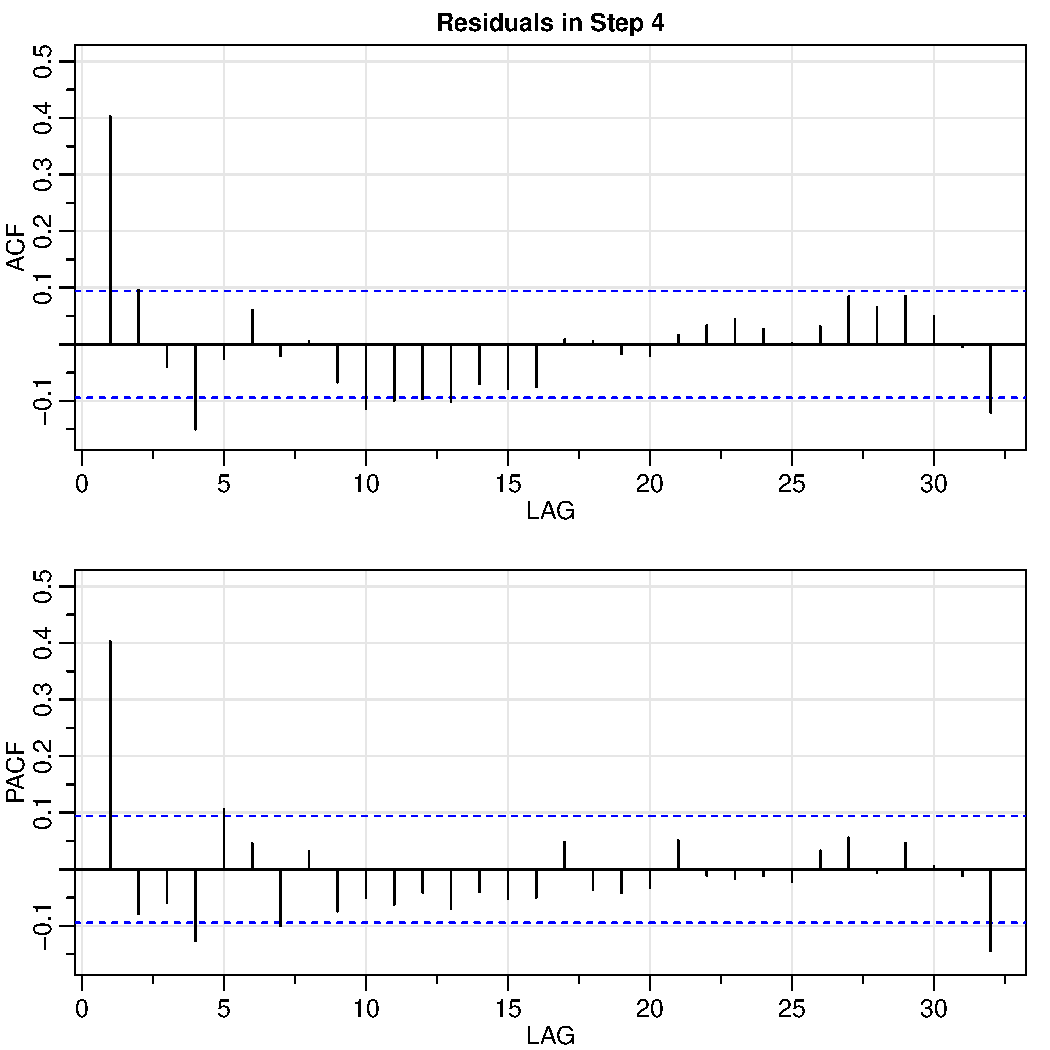
\includegraphics[width=110mm, height=60mm]{residuals_soi.pdf}

Possible structure?

\end{frame}

\begin{frame}
\frametitle{Worked Example}

Fit the (lagged) regression model and specify the ARMA structure of the residuals.

\end{frame}

\begin{frame}
\frametitle{Worked Example}

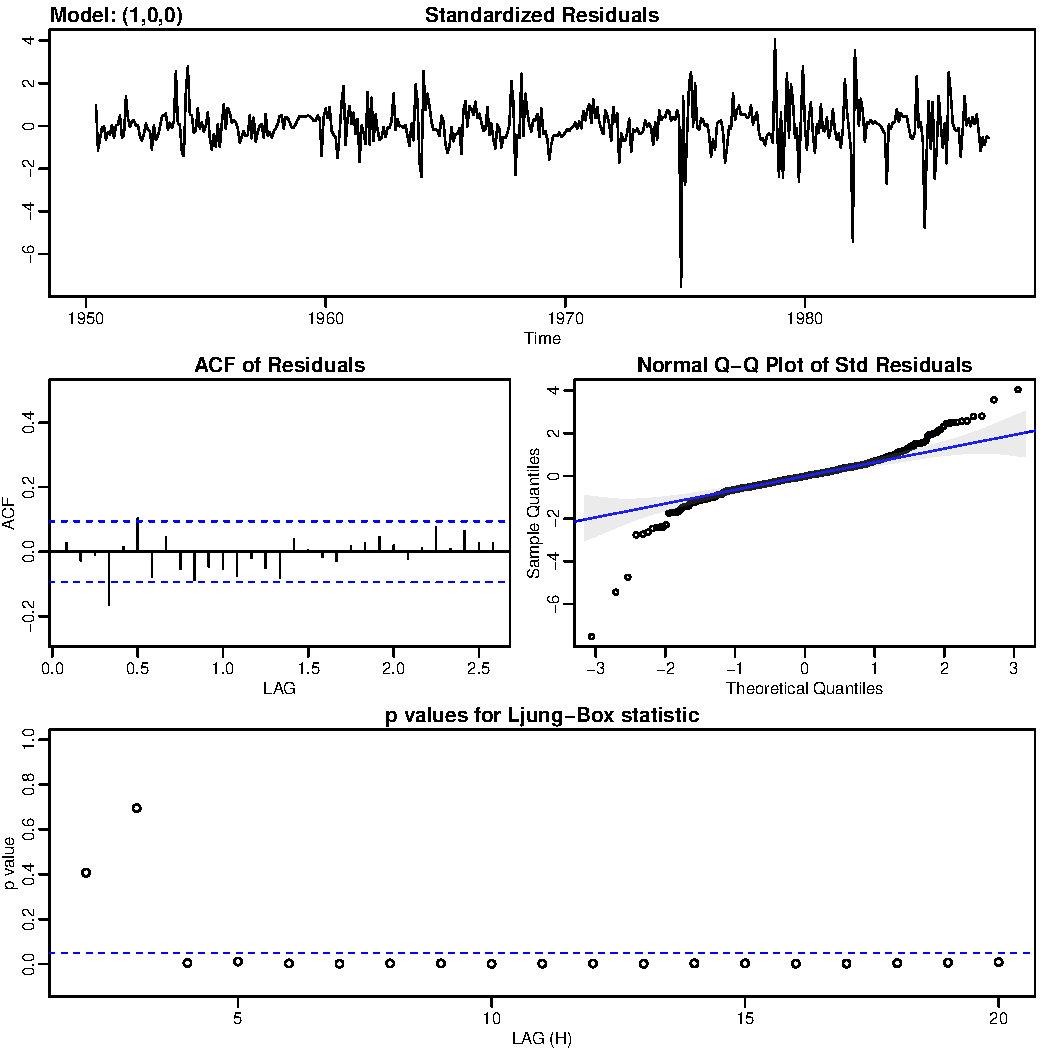
\includegraphics[width=110mm, height=75mm]{diag1.pdf}

\end{frame}

\begin{frame}
\frametitle{Worked Example}

When we think we want to choose a model, make sure to examine the residuals to ensure they appear to be white. Ljung-Box statistics should be insignificant.

\end{frame}

\begin{frame}
\frametitle{Worked Example}

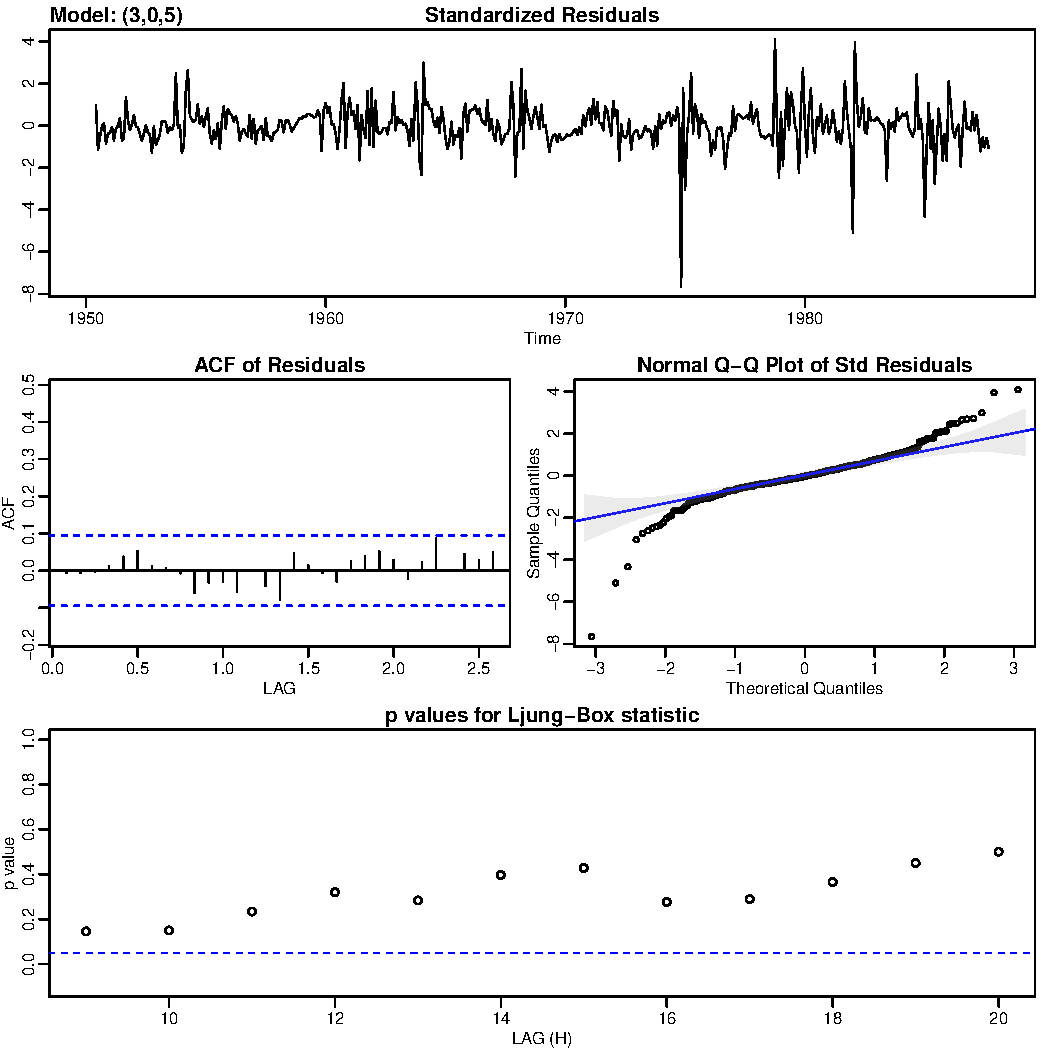
\includegraphics[width=110mm, height=75mm]{diag2.pdf}


\end{frame}

\begin{frame}
\frametitle{Worked Example}

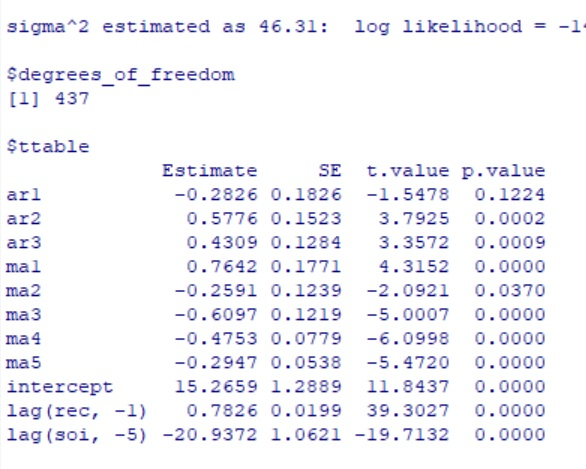
\includegraphics[width=110mm, height=75mm]{lagreg.jpg}



\end{frame}






\end{document} 